\chapter{Prise en main}\label{cha:quickstart}

Ce chapitre montre l'utilisation classique de XCSoar lors de vols sur la campagne. Il est constitué de différents scénarios simples démontrant l'utilisation des fonctionnalités de base du logiciel. Les paramétrages des différentes options utilisateur doivent avoir été faits.

Les exemples fournis constituent une aide "pas à pas" de différents niveaux mais ne sont pas là pour démontrer  l'intégralité des fonctionnalités de XCSoar. De plus, avec de l'expérience, le logiciel peut être utilisé de façon différente et tout aussi efficace.

\section{Le vol local}\label{sec:local-flight}

Dans ce scénario, le pilote a l'intention de voler en local de son terrain ou d'effectuer un vol sur la campagne, occasionnel, sans avoir défini de circuit au préalable.

\subsection*{Avant le décollage}
\begin{enumerate}
\item  Démarrer le logiciel.
\item  A l'aide de \bmenug{Config.}\blink\bmenug{Configuration de vol} entrer les valeurs de ballast (en litres / kg si le poids du pilote doit être pris en compte) et de dégradation de la polaire due aux moucherons ou à la pluie. Sortir du menu Config.
\item  Si aucun circuit n'est utilisé, XCSoar prend automatiquement la position de décollage comme point d'arrivée (voir section~\ref{sec:Goto-tasks}). 
\end{enumerate}

\subsection*{En vol}
\begin{enumerate}
\item  Quand vous le souhaitez, choisissez le calage du MacCready manuellement à partir du menu 
\bmenug{Config.}\blink\bmenug{MacCready $+$/$-$} ou à partir du variomètre.
\item  Modifiez les valeurs Ballast / Moucherons si nécessaire.
\item  Tant que la flèche (à gauche de l'écran) est verte pointant vers le haut, le planeur peut rejoindre sa "maison": il est en local.
\item  Vous pouvez activer le mode  \bmenug{MacCready Auto}quand vous voulez rentrer au point de départ. Si le MC est réglé sur "Arrivée" ou sur "Les 2" alors le calculateur affichera la vitesse optimale pour rejoindre votre "maison".
\end{enumerate}

\subsection*{Après l'atterrissage}
\begin{enumerate}
\item Le menu \bmenug{Info. 2}\blink\bmenug{Etats}vous permet de voir entre autre le temps de vol.
\item Le menu \bmenug{Info. 1}\blink\bmenug{Analyses}vous permet d'analyser votre vol ou de le revoir. 
\item  Le logger IGC vous permet de rejouer le vol.
\item Toutes ces fonctions peuvent être accessibles une fois l'appareil éteint, les données étant stockées.
\end{enumerate}

\section{Circuit FAI}\label{sec:fai-task}

Dans ce scénario, le pilote effectue un triangle FAI, avec un seul secteur de départ. Le passage d'un point de virage.au suivant est automatique.

\subsection*{Avant le décollage}
\begin{enumerate}
\item  Démarrer le logiciel.. 
\item  A l'aide de \bmenug{Config.}\blink\bmenug{Configuration de vol}entrer les valeurs de ballast et de dégradation due aux moucherons ou à la pluie. Entrer la température maximale prévue au sol. Sortir du menu Config.
\item  A l'aide de \bmenug{Nav.}\blink\bmenug{Circuit}et de l'onglet "General" puis \button{Nouveau circuit}créer un nouveau circuit vide. Sélectionner "Insignes / records FAI"  comme type de circuit.
\item A l'aide de "Pts de virage" sélectionner le point de départ.dans la liste et modifier son type en "Quadrant de départ FAI". Fermer le panel.
\item Appuyer sur "Ajouter un point de virage". Sélectionner, dans la liste, le premier point de virage du circuit et modifier son type pour "Quadrant FAI".
\item Faire de même pour le second point de virage. Une bonne chose pour sélectionner le prochain point de virage est de filtrer la liste des points de virage par rapport à un cap et/ou une distance (par rapport au dernier point de virage). 
\item  Faire de même pour définir le point d'arrivé et son type. 
\item Le circuit est défini. Vérifier que tout est bien correct pour un triangle FAI: dans la fenêtre récapitulative des points de virage, un message vous le confirme ou non(Triangle FAI / Triangle non-FAI) 
\item De préférence, enregistrer le circuit en lui donnant un nom facile à se rappeler: Pour cela appuyer sur l'onglet "General" puis \bmenug{Enregistrer.}pour le nommer.
\item Le circuit est enregistré, vous pouvez le déclarer et l'envoyer vers un logger connecté.
\end{enumerate}

\subsection*{En vol}
\begin{enumerate}
\item  Le point de virage courant change automatiquement lors du passage dans les zones de contrôle (en jaune).
\item  Après de début de l'épreuve  \bmenug{Info. 2}\blink\bmenug{Etats}puis onglet "Rules" permet de contrôler la validité du départ (Départ Valide Oui/Non). L'heure de décollage est enregistrée ("Times") ainsi que l'altitude de départ. L'altitude minimum d'arrivée est affichée et calculée en fonction des règles définies.
\item  A chaque instant la flèche noire indique la direction à suivre pour rejoindre, au plus court,  le prochain point de virage tout en intégrant l'effet de la composante du vent de travers sur cette direction.
\item  Si \button{Zoom Auto} est activé, la carte zoomera automatiquement à l'approche des points de virage.
\item Quand vous le souhaitez, caler le MacCready avec le menu, le calculateur ou bien avec le vario connecté ou encore  \button{MC Auto}. Si le MC est réglé sur "Arrivée" ou "Les 2" le calculateur indique la vitesse optimale pour terminer le circuit et la valeur du calage MacCready est la vitesse verticale minimum qu'il faut avoir pour continuer à spiraler (sans perdre de temps). 
\item  Ajuster les valeurs "Ballast" et "Moucherons".
\item  A l'aide de \button{Analyses} vérifiez/contrôlez votre circuit.. 
\item  A l'aide de \button{Etats} regardez le temps écoulé, l'heure estimée d'arrivée, la vitesse moyenne sur le circuit etc...
\item  A tout moment, quand la flèche de vitesse (à gauche de la carte) passe au vert (pointant vers le haut) le planeur peut commencer son arrivée.
\end{enumerate}

\subsection*{Après l'atterrissage}
Voir section~\ref{sec:local-flight}.


\section{Circuit AAT, changement de WPT manuel}\label{sec:aat-task-manual}

Ce scénario décrit un circuit de type AAT avec passage manuel des points de virage.

\subsection*{Avant le décollage}
\begin{enumerate}
\item  Démarrer le logiciel.
\item  A l'aide de \bmenug{Config.}\blink\bmenug{Configuration de vol}entrer les valeurs de ballast et de dégradation due aux moucherons ou à la pluie. Entrer la température maximale prévue au sol. Sortir du menu Config.
\item  A l'aide de \bmenug{Nav.}\blink\bmenug{Circuit}et de l'onglet "General" puis \button{Nouveau circuit}créer un nouveau circuit vide. Sélectionner "AAT"  comme type de circuit.
\item A l'aide de "Pts de virage" sélectionner le point de départ, dans la liste et modifier son type si nécessaire. Fermer le panel.
\item Appuyer sur "Ajouter un point de virage". Sélectionner, dans la liste, le premier point de virage du circuit et modifier son type pour "Cylindre de point de virage" et définir le rayon.
\item Faire de même pour le second point de virage. Une bonne chose pour sélectionner le prochain point de virage est de filtrer la liste des points de virage par rapport à un cap et/ou une distance (par rapport au dernier point de virage). 
\item  Définir le point d'arrivé et son type. 
\item Le circuit AAT est défini. Ouvrir l'onglet "Règles" afin de définir la durée de l'AAT.
\item Avec l'onglet \button{Calculateur} les temps estimés pour réaliser le circuit dans le temps imparti et les distances AAT prévues par XCSoar, sont affichés en faisant varier le calage MC. 
\end{enumerate}

\subsection*{En vol}
\begin{enumerate}
\item Quand le pilote est en l'air et prêt à franchir la ligne de départ, alors appuyer sur \button{Arm
Start}. Le point de virage courant changera automatiquement  pour le suivant une fois dans la zone de départ. Après cela, l'avance automatique est "désarmée". 
% When the pilot is ready to start the task, press the \button{Arm
%Start} button.  The current waypoint will then advance automatically
%once, as the pilot flies through the start sector.  After this occurs, the advance trigger is disarmed.  
\item  Si le pilote souhaite refaire un départ (les faux départs sont assez classiques), il doit revenir manuellement au point de virage précédent (le point de départ ici) en appuyant sur  \button{Start Turnpoint}  et ensuite réarmer  \button{Arm Start} le passage de ligne avant de repasser celle-ci.
%In order to re-start, the pilot needs to manually revert to the
%\button{Start Turnpoint} and again press the \button{Arm Start} button prior to
%flying through the start sector again.
\item  Quand la ligne de départ est passée, appuyer sur  \button{Status}  afin de vérifier que le passage de ligne est bien valide. Si l'heure de départ est affichée, le départ a été détecté et est en accord avec les règles de départ définies dans la configuration du circuit. Sinon, il est affiché ''INVALID''.
%After the task is started, the \button{Status} dialog can be opened to
%verify a valid start was detected. If the start time is given, the start was detected and legal according to 
%the task start rules specified in the configuration.  Otherwise it will display ``INVALID''.
\item  During flight, the estimated elapsed time to complete the task with
different MacCready settings can be explored from the \button{Task Calc} dialog.
Once a decision is made to extend or reduce the AAT range this can be done by
manually manipulate the \button{Target}. This allows the pilot to effectively increase or decrease the task
distance and estimate the consequence in AAT time.

The figure below shows the course around the targets at range set to $-100$\%.
\begin{center}
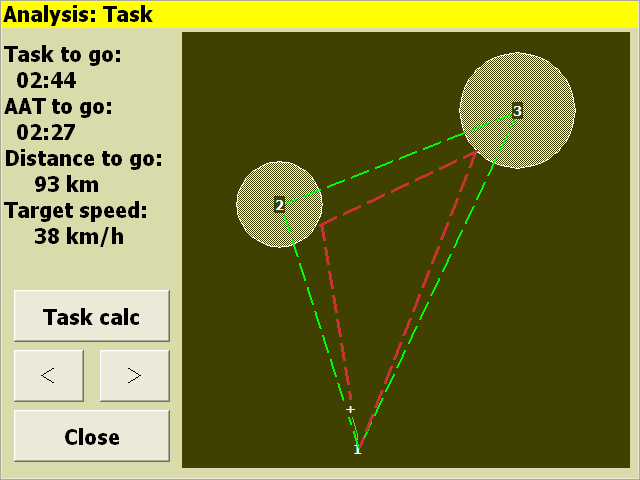
\includegraphics[angle=0,width=0.8\linewidth,keepaspectratio='true']{figures/aat-short.png}
\end{center}

The figure below shows the course around the targets at range set to $100$\%.
\begin{center}
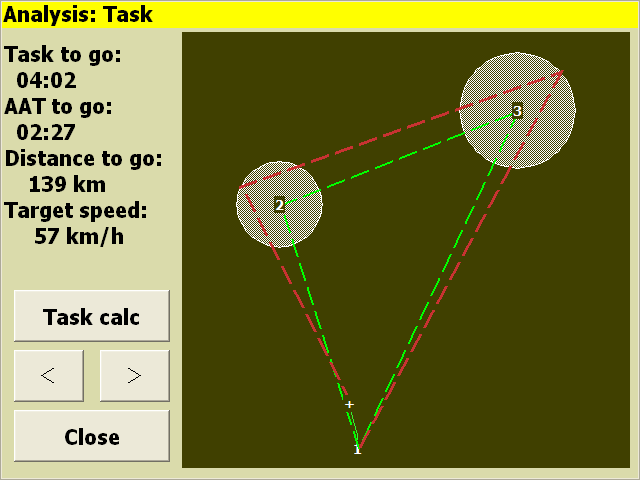
\includegraphics[angle=0,width=0.8\linewidth,keepaspectratio='true']{figures/aat-long.png}
\end{center}

\item  At all times the black track arrow will point at the next target.  The
target is the location within the AAT sector at the range specified in
the \button{Task Calc} dialog.  The blue arrow will point at the direction
the glider should track when in cruise.

\item  When the pilot is within or approaching an AAT sector and is ready to
advance to the next waypoint, press the \button{Arm Turn} button.  The
current waypoint will then advance automatically once, if the pilot is
inside the observation zone.  After this occurs, the advance trigger
is disarmed.

\item If Auto Zoom is activated, the map will automatically zoom in as task waypoints are approached.

\item  At the appropriate times, adjust the MacCready by the menu,
the task calculator or the connected variometer; or activate \button{MC Auto}.
If the MacCready mode was set to `Final Glide' or `Both', then the system will command the optimal 
speed to return home; and the MacCready value will be set to the minimum climb
rate at which it is beneficial to continue to climb.
  
\item  Change the bugs/ballast settings as required.
\item  Refer to the \button{Analysis} dialog as required. 
\item  Refer to the \button{Status} dialog as required.  This shows the start
time, elapsed time on task, estimated arrival time, average task speed etc.
\end{enumerate}

\subsection*{After landing}
As described in Section~\ref{sec:local-flight}.

% Agian in 6.1 
%\section{Task with alternate start sectors}
%
%In this scenario, the pilot intends to fly a task with 
%alternate start sectors and manually arm the waypoint advance system.
%
%\subsection*{Prior to takeoff}
%As described in Section~\ref{sec:fai-task}, except where noted below.
%\begin{enumerate}
%\item Open the `Task edit' dialog, and set `Auto Advance' to `Arm start'.
%  Select the start waypoint, and press enter.  Set `Alternate Start
%  Points' to ON, and press `Edit start points'.  Press `clear' to
%  clear the list of existing start points if required.  Move the
%  cursor to a blank line or `add waypoint' line and press enter; then
%  select the waypoint and press enter.  Repeat for each alternate
%  start point.
%\end{enumerate}
%
%\subsection*{In-flight}
%As described in Section~\ref{sec:fai-task}, except where noted below.
%\begin{enumerate}
%\item 
%Prior to entering the start sector, when the pilot is ready to start
%the task, press the `Arm Advance' button.
%
%\item 
%In order to re-start from any start sector, the pilot needs to press
%the `Arm Advance' button again prior to flying through any of the
%start sectors again.
%\end{enumerate}

